\chapter{\IfLanguageName{dutch}{Stand van zaken}{State of the art}}
\label{ch:stand-van-zaken}

Dit onderzoek is een vergelijkende studie tussen verschillende PostgreSQL oplossingen. In dit hoofdstuk zullen al verschillende oplossingen aan bod komen. Hiermee zal worden gekeken naar de nadruk die gelegd wordt bij elke oplossing. Op deze manier kan gekeken worden naar welke requirements regelmatig terugkomen, en dus welke kunnen gebruikt worden om later in het onderzoek verschillende oplossingen met elkaar te vergelijken. Aan de hand van deze requirements kan geschift worden tussen de bestaande High Availability PostgreSQL cluster oplossingen om hier dan twee oplossingen uit te halen. 

% Tip: Begin elk hoofdstuk met een paragraaf inleiding die beschrijft hoe
% dit hoofdstuk past binnen het geheel van de bachelorproef. Geef in het
% bijzonder aan wat de link is met het vorige en volgende hoofdstuk.
% Pas na deze inleidende paragraaf komt de eerste sectiehoofding.
%Dit hoofdstuk bevat je literatuurstudie. De inhoud gaat verder op de inleiding, maar zal het onderwerp van de bachelorproef *diepgaand* uitspitten. De bedoeling is dat de lezer na lezing van dit hoofdstuk helemaal op de hoogte is van de huidige stand van zaken (state-of-the-art) in het onderzoeksdomein. Iemand die niet vertrouwd is met het onderwerp, weet nu voldoende om de rest van het verhaal te kunnen volgen, zonder dat die er nog andere informatie moet over opzoeken \autocite{Pollefliet2011}.
%Je verwijst bij elke bewering die je doet, vakterm die je introduceert, enz. naar je bronnen. In \LaTeX{} kan dat met het commando \texttt{$\backslash${textcite\{\}}} of \texttt{$\backslash${autocite\{\}}}. Als argument van het commando geef je de ``sleutel'' van een ``record'' in een bibliografische databank in het Bib\LaTeX{}-formaat (een tekstbestand). Als je expliciet naar de auteur verwijst in de zin, gebruik je \texttt{$\backslash${}textcite\{\}}.
%Soms wil je de auteur niet expliciet vernoemen, dan gebruik je \texttt{$\backslash${}autocite\{\}}. In de volgende paragraaf een voorbeeld van elk.
%\textcite{Knuth1998} schreef een van de standaardwerken over sorteer- en zoekalgoritmen. Experten zijn het erover eens dat cloud computing een interessante opportuniteit vormen, zowel voor gebruikers als voor dienstverleners op vlak van informatietechnologie~\autocite{Creeger2009}.

\section{\IfLanguageName{dutch}{PosgreSQL}{PosgreSQL}}
\label{sec:PosgreSQL}

\subsection{\IfLanguageName{dutch}{Databank}{Databank}}
\label{subsec:Databank}

\textcite{Oracle23} omschrijft een databank als een georganiseerde verzameling van gestructureerde informatie, of gegevens, die meestal elektronisch in een computersysteem wordt opgeslagen. Een database wordt gewoonlijk beheerd door een databasebeheersysteem (DBMS). Samen worden de gegevens en het DBMS, samen met de toepassingen die ermee verbonden zijn, een databasesysteem genoemd, vaak afgekort tot gewoon database~\autocite{Oracle23}.

\subsection{\IfLanguageName{dutch}{Relationele Databank}{Relationele Databank}}
\label{subsec:Relationele Databank}

Een relationele databank is een type databank waarin gebruik wordt gemaakt van een structuur die het mogelijk maakt om gegevens te identificeren en te benaderen in relatie tot een ander deeltje data in diezelfde databank. Deze gegevens worden vaak georganiseerd in tabellen. Deze tabellen kunnen honderden, duizenden, miljoenen rijen en kolommen aan data hebben. Een kolom kent vaak ook een specifiek gegevenstype. Deze gegevenstypes kunnen getallen (integers), woorden (strings) of andere soorten bevatten~\autocite{Codecademy}.

\subsection{\IfLanguageName{dutch}{Object-georiënteerde databank}{Object-georiënteerde databank}}
\label{subsec:Object-georiënteerde databank}

Een objectgeoriënteerde database (OODBMS) is een type databank die zich baseert op objectgeoriënteerd programmeren (OOP). De gegevens worden hier voorgesteld en opgeslagen in de vorm van objecten. OODBMS worden ook objectdatabases of objectgeoriënteerde databasemanagementsystemen genoemd~\autocite{CCorner2019}. 

\subsection{\IfLanguageName{dutch}{SQL}{SQL}}
\label{subsec:SQL}

SQL (structured query language) is de eigen programmeertaal specifiek ontwikkelt voor interactie met databanken. Een databank modelleert entiteiten uit het echte leven en slaat deze op in tabellen. Via SQL is het mogelijk om de gegevens in deze tabellen te manipuleren~\autocite{Carchedi2020}. SQL wordt door bijna alle relationele databanken gebruikt zoals MySQL, PostgreSQL, OracleDB, SQLite...~\autocite{Codecademy}. 

\subsection{\IfLanguageName{dutch}{Object-relationele databank}{Object-relationele databank}}
\label{subsec:Object-relationele databank}

Een object-relationele database (ORD / ORDBMS) is een samenstelling uit zowel een relationele database (RDB / RDBMS), als een object-georiënteerde database (OOD / OODBMS). Samen ondersteunt het de basiscomponenten van elk objectgeoriënteerd databasemodel in zijn schema's en gebruikte querytaal, zoals klassen, overerving en objecten. Het bevat aspecten en kenmerken van bovenstaande genoemde modellen. Zo wordt het relationele duidelijk in de manier van opslaan van gegevens. Deze worden opgeslagen in een traditionele database en worden dan met behulp van SQL query's gemanipuleerd en benaderd. Aan de andere kant is ook het objectgeoriënteerde gedeelte merkbaar, namelijk dat de database beschouwd wordt als een objectopslag. Kort gezegd is één van de voornaamste doelstellingen van een object-relationele database, het dichten van de kloof tussen relationele en objectgeoriënteerde modelleringstechnieken en conceptuele datamodelleringstechnieken zoals daar zijn het entiteit-relatiediagram (ERD) en object-relationeel mappen (ORM)~\autocite{Technopedia2021}. %(https://www.techopedia.com/definition/8714/object-relational-database-ord).
%Hieronder bij klasses en overerving kan er al een foto bij ter verduidelijking.
Klasses, Overerving, Types, Functies zijn kenmerken van de object-relationele database en zullen de basisconcepten vormen voor PostgreSQL. Een klasse is een verzameling van gegevenstypes die bij eenzelfde soort iets horen. Bijvoorbeeld een klasse CD kan als kenmerken hebben: Titel, zanger, Datum uitgave, aantal liedjes... . Overerving is wanneer een klasse bepaalde kenmerken overerft, krijgt van een superklasse. Bijvoorbeeld een klasse Fiets erft van de klasse Vervoermiddel de nodige kenmerken. Hierin is de klasse Fiets een specialisatie van de klasse Vervoermiddel. Zo is een kenmerk van de klasse Vervoermiddel het aantal wielen. Dit datatype wordt dan overgeerfd naar de klasse Fiets, waar de invulling van dit datatype twee is. Bij de klasse Auto heeft het overgeerfde kenmerk vier wielen dan. Een type is hierboven al eens genoemd geweest. Dit gaat over de verschillende soorten data die er zijn. Getallen, woorden, objecten zijn hier voorbeelden van. Functies zijn een reeks SQL-statements die een specifieke taak uitvoeren. Functies bevorderen de herbruikbaarheid van code.


\begin{figure}[!h]
    \centering
    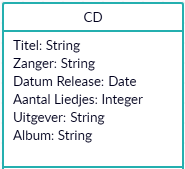
\includegraphics[width=0.25\textwidth]{CD.png}
    \caption{Voorbeeld klasse CD}
    \label{fig:Voorbeeld klasse CD}
\end{figure}

\begin{figure}[!h]
    \centering
    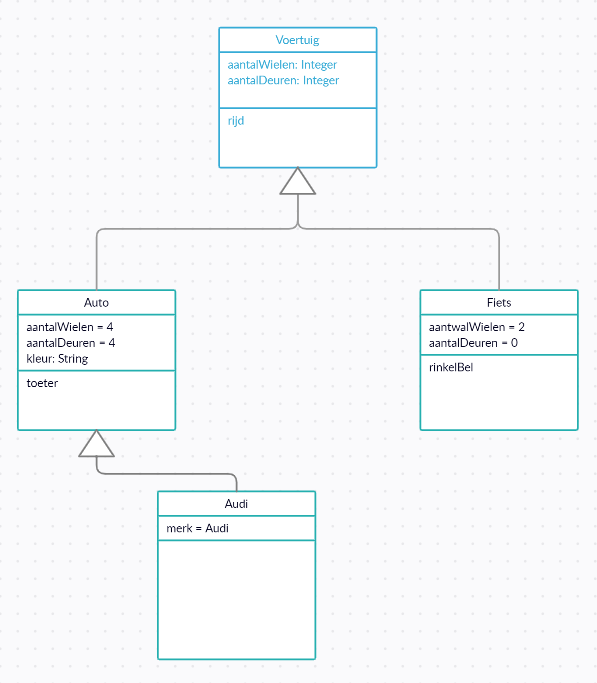
\includegraphics[width=0.75\textwidth]{overerving.png}
    \caption{Voorbeeld overerving}
    \label{fig:Voorbeeld overerving}
\end{figure}
%\textbf{Voorbeeld klasse CD}
%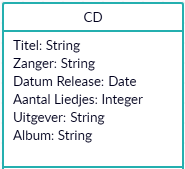
\includegraphics[width=2.5cm]{CD.png}\\[.5cm]

%\textbf{Voorbeeld overerving}
%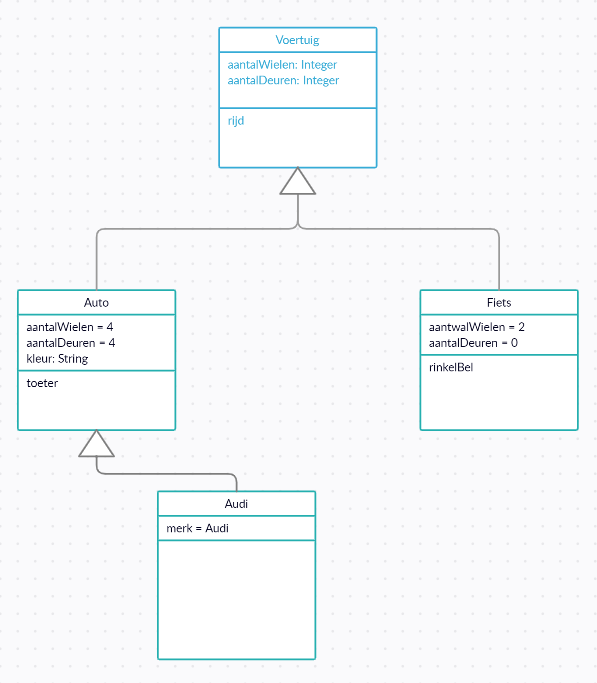
\includegraphics[width=2.5cm]{overerving.png}\\[.5cm]

\subsection{\IfLanguageName{dutch}{PostgreSQL}{PostgreSQL}}
\label{subsec:PostgreSQL}

% https://books.google.be/books?hl=en&lr=&id=Xj85DwAAQBAJ&oi=fnd&pg=PT7&dq=edb+postgres&ots=lQpSIYvp9i&sig=zv5WtrgnlNVxlyzzYFirRvkUf2o#v=onepage&q&f=false

PostgreSQL is een open source systeem dat zich toelegt op het beheer van object-relationele databases. Het heeft meer dan 30 jaar actieve ontwikkeling en heeft een sterke reputatie op vlak van betrouwbaarheid, robuustheid van functies en prestaties~\autocite{postgres}. PostgreSQL biedt een uitgebreide set van functionaliteiten die een hoge mate van customisatie mogelijk maakt binnen het systeem. Dit gaat van data administratie, beveiliging, tot backup en herstel . PostgreSQL wordt regelmatig bijgewerkt door de PostgreSQL Global Development Group en bijdragers uit de community. Deze community ondersteunt zichzelf en zijn gebruikers door het aanbieden van online educatieve bronnen en communicatiekanalen, zoals daar zijn PostgreSQL wiki, online forums en officiële documentatie. Er zijn ook bedrijven die commerciële support bieden aan een prijs~\autocite{Nethosting2019}. Volgens DB-Engines is PostgreSQL de vierde database die vandaag de dag het meest gebruikt wordt en de tweede meest gebruikte open source database, na MySQL~\autocite{DBEngines2021}. DB-Engines verklaarde PostgreSQL in 2017, 2018 en 2020 het DBMS (Database management system) van het jaar~\autocite{DBEngines2021a}.
PostgreSQL biedt veel mogelijkheden om ontwikkelaars te helpen bij het bouwen van applicaties; om beheerders te helpen bij het beschermen van data-integriteit; en bij het bouwen van fouttolerante omgevingen. Het helpt ook bij het beheren van data, hoe groot of hoe klein de dataset ook is. PostgreSQL voldoet sinds september 2020 aan 170 van de 179 verplichte functies voor SQL:2016 Core conformiteit. Schaalbaarheid valt ook toe te schrijven aan PostgreSQL, dit zowel in de hoeveelheid data die het kan beheren, als in het aantal gelijktijdige gebruikers dat het kan accomoderen. Er zijn actieve PostgreSQL clusters in productie omgevingen die terabytes aan data beheren, en gespecialiseerde systemen die zelfs petabytes beheren~\autocite{PostgreSQL2021}. Enkele voorbeelden om te tonen hoe schaalbaar PostgreSQL wel is.

Postgres speelt in op de bovenvernoemde vier basisconcepten van een object-relationele databank zodat gebruikers het systeem makkelijk kunnen uitbreiden. Deze vier kenmerken, naast nog andere functies maken van Postgres een object-relationele database. Bovenstaande vermelde kenmerken zouden doen blijken dat Postgres voornamelijk een object-georiënteerde database is, maar de ondersteuning van de traditionele relationele databases, toont duidelijk aan dat, ondanks de object-georiënteerde kenmerken, Postgres stevig verankerd is in de relationele database wereld ~\autocite{PostgreSQL2021a}.




\section{\IfLanguageName{dutch}{High Availability}{High Availability}}
\label{sec:High Availability}

Het doel van High Availability architectuur is ervoor te zorgen dat een server, website of applicatie verschillende vraagbelastingen en verschillende soorten storingen kan verdragen. En dit met de minst mogelijke downtime. Door gebruik te maken van best practices die zijn ontworpen om hoge beschikbaarheid te garanderen, helpt dit volgens \textcite{Australia2017} om in een organisatie maximale productiviteit en betrouwbaarheid te bereiken~\autocite{Australia2017}. 

% niet elke situatie vereist high availability, wanneer is dit nodig dan?

% Waarom is dit nodig?
% Wat zijn de mogelijkheden om hieraan te voldoen? en Hoe implementeert postgres deze oplossingen

High Availability is het vermogen van een systeem om continu operationeel te blijven te zijn gedurende een wenselijk lange tijd. Men kan Availability meten ten opzichte van 100\% operationeel, als in, nooit uitvallen. Beschikbaarheid wordt vaak uitgedrukt als een percentage van uptime in een bepaald jaar op basis van de SLA's, Service Level Agreements ~\autocite{Kumar2020}. Vaak duidt men deze norm aan als de Five 9's, namelijk 99,999\% beschikbaarheid~\autocite{Lutkevich2021}. High availability impliceert dat delen van een systeem volledig zijn getest en dat er voorzieningen zijn voor storingen/failures in de vorm van redundante componenten. Servers kunnen worden ingesteld om in geval van nood de verantwoordelijkheden over te dragen aan een externe server, in een back-up proces. Hier spreekt men dan van failover ~\autocite{Technopedia2021a}.

% https://www.postgresql.org/docs/9.5/high-availability.html Deze link nog eens uitspitten
Wanneer is High Availability nu eigenlijk nodig?
High Availability is nuttig wanneer bedrijven te maken hebben met dagelijk kritisch applicatiebeheer. Of wanneer er veel traffiek is op de website, is het niet te veroorloven om downtime te hebben. Een simpele reden als gewoon goede service aanbieden, is ook een geldige reden om aan High Availability te doen~\autocite{CriticalCase2020}. 


Belangrijke principes van High Availability zijn:

1. \textbf{Het elimineren van single point of failure}: Toevoeging van redundantie zorgt er voor zodat het falen van een onderdeel in het systeem niet leidt tot het volledige falen van een geheel systeem.

2. \textbf{Betrouwbare cross-over}: In een redundant systeem wordt het kruispunt zelf een single point of failure. Fouttolerante systemen moeten voorzien in een betrouwbaar crossover- of automatisch omschakelingsmechanisme om storingen te voorkomen.

3. \textbf{Storingdetectie}: Als bovenstaande principes proactief bewaakt worden, dan zal een gebruik misschien nooit een systeemstoring zien.
Postgres biedt de bouwstenen om bovenstaande principes volledig uit te werken zodat er op deze manier High Availability verzekerd kan worden.

Bij het elimineren van single points of failure ondersteunt Postgres de volgende fysieke stand-by's:

1. \textbf{Cold Standby}: Dit is een back-up server die beschikt over back-ups en alle nodige WAL-bestanden voor herstel. WAL is de afkorting voor Write Ahead Log. Het logt elke transactie die uitgevoerd wordt op een database voordat het wordt uitgevoerd. Een Cold Standby systeem is geen operationeel systeem, maar het kan wel beschikbaar worden gemaakt als dat nodig is. Voornamelijk worden dan backup servers en WAL bestanden gebruikt voor het maken van een nieuwe PostgreSQL node als onderdeel van disaster recovery.

2. \textbf{Warm Standby}: Hierin draait Postgres in herstelmodus en ontvangt updates door gebruik te maken van gearchiveerde logbestanden of door gebruik te maken van log shipping replicatie van Postgres. Log shipping is een proces waarbij de back-up van transactielogbestanden op een primaire database wordt geautomatiseerd en vervolgens op een standby server wordt hersteld~\autocite{Miller2016}. In deze modus aanvaardt Postgres geen verbindingen en queries.

3. \textbf{Hot Standby}: Ook bij Hot Standby draait Postgres in herstelmodus en ontvangt het updates door gebruik te maken van gearchiveerde logbestanden of door gebruik te maken van log shipping van Postgres. Het verschil met Warm Standby is dat in deze herstelmodus Postgres hier wel verbindingen ondersteunt en read-only queries.

Bovenstaande voorbeelden zijn mogelijkheden die kunnen helpen bij het elimineren van single points of failure. Afhankelijk van het overeengekomen niveau van beschikbaarheid, kunnen gebruikers voor een van de bovenstaande kiezen.

In geval van een volledige uitval van een systeem is geografische redundantie algemeen zeer wenselijk. Op deze manier worden servers verdeeld over meerdere locaties verdeeld over de wereld. Bij downtime door een natuurramp bijvoorbeeld zijn standby servers op meerdere fysieke (ongetroffen) locaties beschikbaar om in te vallen. Dit type van redundantie kan zeer duur uitdraaien, waarbij het een verstandige beslissing kan zijn om te kiezen voor een gehoste oplossing, waarbij de provider datacenters heeft over heel de wereld.

\subsection{\IfLanguageName{dutch}{Load Balancing}{Load Balancing}}
\label{subsec:Load Balancing}

Load Balancing is ook een manier om High Availability te waarborgen. Het doel van een load balancer is om toepassingen en/of netwerkverkeer te verdelen over meerdere servers en componenten. Het zal binnenkomende verzoeken routeren naar verschillende servers. Hiermeer wil het optionele prestaties en betrouwbaarheid verbeteren. Enkele voorbeelden van load balancing is Round Robin die ervoor zorgt dat de verzoeken van de load balancer naar de eerste server gaan in de rij. De verzoeken gaan deze rij af, tot hij op het einde komt, waarna hij terug van het eerste element in de rij begint. Een tweede manier van load balancing is Least Connection. Hierbij zal er gekozen worden om gebruik te maken van de server met het minst aantal actieve verbindingen. Load balancers spelen een rol bij het tot stand brengen van een infrastructuur met High Availability, maar het hebben van een load balancer staat niet garantie voor het hebben van High Availability. Door redundantie te implementeren voor de load balancer zelf, kan deze geelimineerd worden als een single point of failure~\autocite{Jevtic2018})

HAProxy, High Availability Proxy, is hier een voorbeeld van. Dit is een op software gebaseerde TCP/HTTP load balancer. Het verdeelt de werklast over meerdere servers zodat het prestaties kan maximaliseren en het gebruik van resoucres kan optimaliseren~\autocite{SeveralNines2020}.

\subsection{\IfLanguageName{dutch}{Schaalbaarheid}{Schaalbaarheid}}
\label{subsec:Schaalbaarheid}

Schaalbaarheid is de eigenschap van een systeem om te kunnen voldoen aan een groeiend aantal eisen door bronnen toe te voegen. De redenen voor een groei kunnen tijdelijk zijn, bijvoorbeeld wanneer een bedrijf net een nieuw product op de markt brengt, of wanneer er een substantiële groei is in het aantal klanten of personeel. Er zijn twee manieren om aan schalen te doen. Horizontaal en verticaal~\autocite{Insausti2019}.

\subsubsection{\IfLanguageName{dutch}{Horizontaal schalen}{Horizontaal schalen}}
\label{subsubsec:Horizontaal schalen}
Horizontaal schalen richt zich op het toevoegen van nodes in een systeem of cluster. Hierin is het handig om meer slave nodes toe te voegen aan de cluster. Dit zal helpen om lees- en schrijfprestaties te verbeteren, doordat het meer gebalanceerd kan gebeuren. Hierbij is een load balancer nodig, die dit verkeer zal regelen. Eén load balancer zal niet voldoende zijn om single point of failure preventief te voorkomen. Beter hier is dan twee of meerdere load balancers toevoegen. Op deze manier blijft High Availability een garantie~\autocite{Insausti2019}.

\subsubsection{\IfLanguageName{dutch}{Verticaal schalen}{Verticaal schalen}}
\label{subsubsec:Verticaal schalen}
Verticaal schalen is het toevoegen van hardware resources aan bestaande nodes. Deze resources kunnen gaan over RAM-geheugen, schijfgeheugen, CPU~\autocite{Insausti2019}.

\section{\IfLanguageName{dutch}{Cluster oplossingen}{Cluster solutions}}
\label{sec:Cluster solutions}

\subsection{\IfLanguageName{dutch}{Cluster}{Cluster}}
\label{subsec:Cluster}

Een cluster is een groepering van servers die met elkaar samenwerken om één geheel te vormen. Op deze manier kan een cluster High Availability mogelijk maken~\autocite{TechTarget2017}.

\subsection{\IfLanguageName{dutch}{Failover}{Failover}}
\label{subsec:Failover}

Failover is het automatisch overschakelen naar een back-upsysteem. Wanneer een primair systeemonderdeel faalt, wordt failover ingeschakeld om de negatieve gevolgen te elimineren of te beperken~\autocite{AVINetworks2020}.

\subsection{\IfLanguageName{dutch}{Failback}{Failback}}
\label{subsec:Failback}

Failback is het proces van het herstellen van operaties naar een primaire machine  nadat ze zijn verschoven geweest naar een secundaire machine wegens failover~\autocite{TechTarget2020}.

\subsection{\IfLanguageName{dutch}{Patroni}{Patroni}}
\label{subsec:Patroni}

%https://www.cybertec-postgresql.com/en/services/postgresql-replication/high-availability-patroni/

Patroni is een open source cluster-technologie, geschreven in Python die zich bezighoudt met automatische failover en High Availability voor een PostgreSQL databank. Het dient als een soort cluster manager die de implementatie en het onderhoud van High Availability in PostgreSQl clusters zal aanpassen en automatiseren. Het maakt gebruik van gedistribueerde configuratieopslagplaatsen zoals etcd, Consul, ZooKeeper of Kubernetes voor maximale toegankelijkheid~\autocite{Markwort2018}.


Patroni biedt cloud-native netwerkfuncties en geavanceerde opties voor failback en failover. Een cloud-native netwerkfunctie is een software-implementatie van een netwerkfunctie, die wordt uitgevoerd in een linux-container, die traditioneel wordt uitgevoerd door een fysiek apparaat~\autocite{CDNF2020}.

Als oplossing zorgt Patroni voor een end-to-end setup van High Available PostgreSQL clusters, inclusief streaming replicatie. Streaming replicatie biedt de mogelijkheid om continu WAL logs naar standby servers te sturen en deze toe te passen om de servers op deze manier up to date te houden~\autocite{2020}. %(https://wiki.postgresql.org/wiki/Streaming_Replication#:~:text=Streaming%20Replication%20(SR)%20provides%20the,some%20out%20of%20date%20information) 
Het biedt verschillende manieren waarop een standby node kan aangemaakt worden, en dient als sjabloon dat kan worden aangepast naar wat gewenst word.

Bij het aanmaken van een standby node maakt Patroni gebruik van pg\_basebackup en ondersteunt het ook methodes zoals Barman, pgBackRest en meer die gebruikt worden voor het aanmaken van standby nodes.

Na het opzetten van de cluster, zal Patroni zich actief bezighouden met het monitoren. Patroni zal werken aan de hand van een leader lock. Deze wordt om de zoveel tijd vernieuwt, en wanneer de master node er niet in slaagt om deze te vernieuwen, zal Patroni een nieuwe node verkiezen tot master node~\autocite{ScaleGrid2018}. %(https://scalegrid.io/blog/managing-high-availability-in-postgresql-part-3/#:~:text=Patroni%20ensures%20the%20end%2Dto,be%20customized%20to%20your%20needs.)

%https://buildmedia.readthedocs.org/media/pdf/patroni/latest/patroni.pdf
%https://blog.dbi-services.com/postgresql-high-availabilty-patroni-ectd-haproxy-keepalived/

\subsection{\IfLanguageName{dutch}{Pgpool-II}{Pgpool-II}}
\label{subsec:Pgpool-II}

%https://www.pgpool.net/mediawiki/index.php/Main_Page

Pgpool-II omschrijft zichzelf als een middleware die werkt tussen PostgreSQL servers en een PostgreSQL database client. Het ondersteunt High Availability, geautomatiseerde load balancing, etc. Pgpool-II biedt ook logical replication. Logische replicatie, of logical replication stelt gebruikers in staat om een selectieve replica van bepaalde tabellen uit te voeren en deze uit te schrijven naar een standby node. Met logical replication kan een standby node replicatie ingeschakeld hebben van meerdere master nodes. Dit kan handig zijn in situaties waar je gegevens van verschillende PostgreSQL databases moet repliceren naar een enkele PostgreSQL server voor rapportage en data warehousing. Eén van de grootste voordelen van logische replication boven streaming replication is dat logical toelaat om veranderingen van een oudere versie van PostgreSQL naar een nieuwere versie te repliceren. Streaming replicatie werkt alleen als zowel de master als de standby van dezelfde versie zijn. Wat niet altijd ideaal is in grote opstellingen~\autocite{Vallarapu2019}. %(https://www.percona.com/blog/2019/04/04/replication-between-postgresql-versions-using-logical-replication/#:~:text=Logical%20replication%20in%20PostgreSQL%20allows,is%20not%20open%20for%20writes.) 
Pgpool-II biedt de volgende features:

1. Connection Pooling

Pgpool-II bewaart verbindingen naar de PostgreSQL servers, en hergebruikt ze wanneer een nieuwe verbinding met dezelfde eigenschappen zoals gebruikersnaam, database of protocol versie binnenkomt. Dit vermindert de overhead van verbindingen, en verbetert de totale doorvoer van het systeem.

2. Replication

Pgpool-II kan meerdere PostgreSQL servers beheren. Door gebruik te maken van de replicatiefunctie kan een realtime backup worden gemaakt op 2 of meerdere fysieke schijven, zodat de dienst kan worden voortgezet zonder servers te stoppen in geval van een schijfstoring.

3. Load Balancing

Als een database wordt gerepliceerd, zal het uitvoeren van een query op elke server hetzelfde resultaat opleveren. Pgpool-II maakt gebruik van de replicatie mogelijkheid om de belasting op elke PostgreSQL server te verminderen door queries over meerdere servers te verdelen, waardoor de totale throughput van het systeem verbetert. In het meest gunstige geval verbetert de prestatie evenredig met het aantal PostgreSQL servers. Load balance werkt het beste in een situatie waarin er veel gebruikers zijn die veel queries tegelijkertijd uitvoeren.

4. Limiting Exceeding Connections

Er is een limiet op het maximum aantal gelijktijdige verbindingen met PostgreSQL, en verbindingen worden geweigerd na dit maximaum aantal verbindingen. Het instellen van een max aantal verbindingen verhoogt echter het verbruik van bronnen en beïnvloedt de systeemprestaties. pgpool-II heeft ook een limiet op het maximum aantal verbindingen, maar extra verbindingen worden dan in een wachtrij geplaatst..

5. Watchdog

Watchdog kan een robuust clustersysteem creëren en het single point of failure of split brain vermijden. Watchdog kan een lifecheck uitvoeren tegen andere Pgpool-II nodes, om een fout van Pgpool-II te detecteren. Als actieve Pgpool-II down gaat, kan dan een standby Pgpool-II gepromoveerd worden tot actief, en zal deze dan virtueel het IP overnemen.

6. In Memory Query Cache

In memory query cache maakt het mogelijk om een paar SELECT statements en zijn resultaat op te slaan. Als een identieke SELECT binnenkomt, retourneert Pgpool-II de waarde uit de cache. Omdat er geen SQL parsing of toegang tot PostgreSQL aan te pas komt, is het gebruik van in memory cache extreem snel. Aan de andere kant kan het in sommige gevallen langzamer zijn dan het normale pad, omdat het wat overhead toevoegt van het opslaan van cache gegevens.

Pgpool-II praat met de backend en de frontend protocollen van PostgreSQL, en legt een verbinding tussen beide. Daarom denkt een database applicatie (frontend) dat Pgpool-II de eigenlijke PostgreSQL server is, en de server (backend) ziet Pgpool-II als een van zijn clients. Omdat Pgpool-II transparant is voor zowel de server als de client, kan een bestaande databasetoepassing met Pgpool-II worden gebruikt vrijwel zonder de broncode aan te passen~\autocite{2021}. %(https://www.pgpool.net/mediawiki/index.php/Main_Page)


\subsection{\IfLanguageName{dutch}{PostgreSQL Automatic Failover (PAF)}{PostgreSQL Automatic Failover (PAF)}}
\label{subsec:PostgreSQL Automatic Failover (PAF)}

PostgreSQL Automatic Failover (PAF) is een nieuwe resource agent, speciaal voor PostgreSQL. Door Pacemaker en Corosync, is het voor PAF mogelijk om:

1. Aan detectiestoring te doen van een PostgreSQL instance.

2. de primary server te herstellen...

3. of om aan failover te doen naar een standby server.

4. Om de best (met de kleinste vertraging) beschikbaarste standby server te selecteren bij failover.

5. Rollen te wisselen in de cluster tussen standby en primary nodes.


De oorspronkelijke wens is om een duidelijke grens te houden tussen de Pacemaker administratie en de PostgreSQL administratie, om dingen eenvoudig, gedocumenteerd en toch krachtig te houden.

Zodra een PostgreSQL cluster is opgebouwd met behulp van interne streaming replicatie, is PAF in staat om aan Pacemaker te laten zien wat de huidige status is van de PostgreSQL instantie op elke node: primary, standby, gestopt, etc. Mocht er dan een storing optreden op de primary node, dan zal Pacemaker standaard proberen deze te herstellen. Mocht de storing niet te herstellen zijn, dan zorgt PAF ervoor dat de standby servers de beste van hen kunnen kiezen (de dichtstbijzijnde bij de oude primary) en deze promoveren tot de nieuwe primary. Dit doet PAF dankzij Pacemaker~\autocite{Rimbault2020}. %(https://clusterlabs.github.io/PAF/)

Postgres Automatic Failover (PAF) biedt verschillende voordelen in het omgaan met PostgreSQL High Availability. PAF gebruikt IP adres failover in plaats van het herstarten van de standby om verbinding te maken met de nieuwe master tijdens een failover event. Dit blijkt voordelig te zijn in scenario's waarbij de gebruiker de standby nodes niet opnieuw wil opstarten. PAF heeft ook zeer weinig manuele tussenkomst nodig en beheert de algemene gezondheid van alle Postgres databankbronnen. Het enige geval waarin manuele tussenkomst een vereiste is, is dan in het geval van een tijdlijn data divergentie waarbij de gebruiker kan kiezen om pg\_rewind te gebruiken~\autocite{ScaleGrid2018a}. Pg\_rewind is een tool die helpt bij het synchroniseren van een PostgreSQL cluster met een andere kopie van diezelfde cluster, met als enige verschil de tijd. Voorbeeld hierbij is een oude master node terug online brengen na failover als een standby node die de nieuwe master node volgt~\autocite{PostgreSQL2021b}. %(https://www.postgresql.org/docs/12/app-pgrewind.html)

\subsection{\IfLanguageName{dutch}{RepMgr [Replication Manager]}{RepMgr [Replication Manager]}}
\label{subsec:RepMgr [Replication Manager]}
%https://wiki.postgresql.org/wiki/Repmgr#repmgr_5_Features

Repmgr is een open-source oplossing die zich bezighoudt met het beheren van replicatie en failover van servers in PostgreSQl clusters. Het verbetert de ingebouwde hot-standby opties van PostgreSQL met extra features zoals tools om standby servers op te zetten, replicatie te monitoren en administratieve taken uit te voeren, zoals failover~\autocite{2021a}. %(https://repmgr.org/)

De features die repmgr 5 aanbiedt zijn:

1. De implementatie als een PostgreSQL extentie.

2. Replicatie cluster monitoring.

3. Standby klonen aan de hand van pg\_basebackup of Barman

pg\_basebackup: pg\_basebackup wordt gebruikt om basisbackups te maken van een draaiende PostgreSQL databank cluster. Deze back-ups worden gemaakt zonder de aanwezige cliënts, die in verbinding staan met de databank, te beïnvloeden. Deze back-ups kunnen gebruikt worden voor zowel point-in-time recovery, maar ook als een startpunt voor log shipping of streaming replicatie standby servers. Bij point-in-time recovery wordt verwezen naar herstel van dataveranderingen tot een bepaald punt in de tijd~\autocite{MySQL2021}. %(https://dev.mysql.com/doc/mysql-backup-excerpt/8.0/en/point-in-time-recovery.html#:~:text=Point%2Din%2Dtime%20recovery%20refers,time%20the%20backup%20was%20made.)

pg\_basebackup maakt een binaire kopie van de database cluster bestanden, terwijl het ervoor zorgt dat het systeem automatisch in en uit backup modus wordt gezet. Backups worden altijd gemaakt van de gehele databasecluster; het is niet mogelijk om een backup te maken van afzonderlijke databases of databaseobjecten. 

De backup wordt gemaakt over een gewone PostgreSQL verbinding maakt gebruik van het replicatieprotocol. De server moet ook worden geconfigureerd om ten minste één sessie beschikbaar te laten voor de backup~\autocite{PostgreSQL2021c}. %(https://www.postgresql.org/docs/10/app-pgbasebackup.html)

Barman: Barman of pgbarman staat voor Backup en Recovery Manager. Het is een open-source beheertool voor disaster recovery van PostgreSQL servers. Het is geschreven in Python. Barman laat toe om van op afstand van meerdere servers in bedrijfskritische omgevingen back-ups uit te voeren. Het helpt ook database beheerders tijdens een herstelfase~\autocite{Barman2020}~\autocite{Barman2020a}. %(https://www.pgbarman.org/about/)(https://www.pgbarman.org/)

4. Standby server die kan worden gepromoveerd tot een primary server zonder herstart. Andere standby servers die verbinding kunnen maken met de nieuwe master zonder opnieuw gesynchroniseerd te worden~\autocite{2020a}.
%https://wiki.postgresql.org/wiki/Repmgr#repmgr_5_Features

5.Cascading Standby Support

Standby servers die niet direct verbonden zijn met de master node worden niet beïnvloed tijdens failover van de primary naar een andere standby mode.

6. Vereenvoudigen van het beheer van WAL-retentie en ondersteuning voor replicatiesleuven

Door de vereenvoudiging van WAL-retentie zal het dus eenvoudiger zijn om WAL-bestanden op te ruimen vanaf elke bestandssysteemlocatie. Ook in standby servers kan het gebruikt worden om bestanden die niet meer nodig zijn, te verwijderen uit de standby server~\autocite{Augustine2019}.
%(https://www.percona.com/blog/2019/07/10/wal-retention-and-clean-up-pg_archivecleanup/)

7. Switchover ondersteuning voor rolswitching tussen primary en standby

Hierin wordt een standby server geprovomeerd tot een primary server en zal deze primary server degraderen naar een standby server. Wanneer andere standby servers verbonden zijn met de degradatiekandidaat, kan repmgr deze instrueren om de nieuwe primary server te volgen en niet de oude, die net gedegradeerd is~\autocite{2021b}. %(https://repmgr.org/docs/4.0/repmgr-standby-switchover.html)

\subsection{\IfLanguageName{dutch}{PgBouncer}{PgBouncer}}
\label{subsec:PgBouncer}

PgBouncer is een open source connection-pooler die gebruikt wordt voor PostgreSQL. Het kan verbindingen naar één of meerdere databases poolen. Het onderhoudt voor een pool van verbindingen per gebruiker. Het wordt vaak geconfigureerd om één van de verbindingen uit te delen aan een nieuwe inkomende cliëntverbinding en terug te geven aan de pool wanneer de cliënt de verbinding verbreekt~\autocite{Ramachandran2019}.

\subsection{\IfLanguageName{dutch}{Raima}{Raima}}
\label{subsec:Raima}

Databasereplicatie is het proces waarin gegevens worden gekopieerd van een database naar één of meerdere replica's. Dit om de toegankelijkheid van gegevens en fouttolerantie te verbeteren.
In de context van replicatie gebruikt men vaak ook de termen actief-actief en actief-passief. Raima Database Manager (RDM) ondersteunt beide technieken. Bij Raima wordt actieve replicatie gewoon replicatie genoemd en passieve replicatie spiegelen (mirroring). Spiegelen zal resulteren in identieke replica's zoals de originele database, terwijl replicatie zal resulteren in replica's die niet identiek zijn aan de originele database. Deze replica's zullen alle records bevatten die van de originele database zijn overgebracht, maar de fysieke organisatie van de records in de databasebestanden (of in het geheugen) kan verschillen.
Om terug te komen op de termen actief-actief en actief-passief zullen die vaker verwijzen naar andere concepten dan dewelke juist omschreven (replicatie en spiegelen). Actieve-actieve replicatie betekent replicatie in twee richtingen van gegevens tussen twee databases die beide actief worden bijgewerkt. Actieve-passieve replicatie betekent replicatie in één richting van een actief bijgewerkte master node naar een slave node die niet wordt bijgewerkt, behalve door het replicatieproces. Hier verwijst men soms ook naar master-slave replicatie. In RDM is replicatie altijd actief-passief~\autocite{Raima2021}. %(https://raima.com/rdme-high-availability-database/).

\subsection{\IfLanguageName{dutch}{EDB}{EDB}}
\label{subsec:EDB}

Voor betrouwbare cross-over biedt EDB een technologie genaamd EDB Postgres Failover Manager (EFM). Dit maakt automatische failover van de Postgres master node naar een standby node mogelijk in geval van een software- of hardwarefout op de master. EFM maakt gebruik van JGroups, die een betrouwbare, gedistribueerde en redundante infrastructuur biedt zonder een single point of failure.
EDB Postgres Failover Manager kan ook gebruikt worden voor de detectie van storingen. Het bewaakt de server continu en zal storingen op verschillende niveaus detecteren. Het is ook capabel om om failover uit te voeren van de master node naar één van de replica nodes om het systeem beschikbaar te maken voor het accepteren van databaseverbindingen en queries. Wanneer EFM goed geconfigureerd is, kan het storingen detecteren en direct failover uitvoeren.

Verlies van service kan in twee categoriëen opdelen. Geplande uitval of downtime en ongeplande uitval of downtime.
Geplande downtime is vaak het gevolg van onderhoudsactiviteiten. Dit kan zijn door een softwarepatches die een herstart van het systeem of van de database vereist. In het algemeen is deze uitval niet onverwachts en zal deze uitval geen grootschalige gevolgen hebben.
Een ongeplande downtime is vaak het resultaat van een of andere fysieke gebeurtenis, zoals hardware- of softwarestoring, of een anomalie in de omgeving. Stroomuitval, defecte CPU- of RAM-componenten (of eventueel andere hardwarecomponenten), netwerkstoringen, inbreuken op de beveiliging, of diverse defecten in toepassingen, middleware en besturingssystemen resulteren bijvoorbeeld in ongeplande uitval.
In geval van (on)geplande downtime kan EFM helpen om de downtime zoveel mogelijk te minimaliseren. Voor een geplande downtime kan een gebruiker bijvoorbeeld eerst alle standby nodes patchen en EFM gebruiken om over te schakelen voordat de master node gepatcht wordt. Bij een ongeplande downtime kan EFM ervoor zorgen dat de storingen gedetecteerd worden en failover uitvoeren naar de juiste standby node, om dan deze node de nieuwe master node te maken. EFM zal na dit proces er ook voor zorgen dat de oude master node niet terugkomt om een split-brain situatie te voorkomen. Split-brain duidt op de inconsistenties in beschikbaarheid en data. Hierdoor ontstaan er twee afzonderlijke datasets met overlap~\autocite{Kumar2020}. %(https://www.enterprisedb.com/blog/what-does-database-high-availability-really-mean).


% (https://wiki.postgresql.org/wiki/Replication,_Clustering,_and_Connection_Pooling)
% (https://wiki.postgresql.org/wiki/Clustering)



\section{\IfLanguageName{dutch}{Puppet}{Puppet}}
\label{sec:Puppet}

Puppet CTO Deepak Giridharagopal zei dat in het kielzog van de economische neergang als gevolg van de COVID-19 pandemie, meer IT-teams zwaar zullen moeten vertrouwen op automatisering. De meeste IT-teams zullen ofwel even groot blijven of worden ingekrompen. De IT-omgeving zal echter steeds complexer worden. De enige manier om IT-teams in staat te stellen meer te doen met minder is het automatiseren van meer routinetaken~\autocite{Vizard2020}. %(https://devops.com/puppet-brings-orchestration-to-it-automation/).

Puppet is een cross-platform client-server gebaseerde toepassing die wordt gebruikt voor configuratiebeheer. Het behandelt de software en zijn configuraties op meerdere servers. Er zijn hierbij twee versies beschikbaar. De ene is open-source, de andere is een betalende, commerciële versie. Het werkt op zowel Linux als op Windows. Het gebruikt een declaratieve aanpak om updates, installaties en andere taken te automatiseren. De software kan systemen configureren met behulp van bestanden die manifesten worden genoemd. Een manifest bevat instructies voor een groep of type server(s) die wordt/worden beheerd~\autocite{Kelly2020}. %(https://www.liquidweb.com/kb/what-is-puppet-and-what-role-does-it-play-in-devops/). 

Wat is configuratiebeheer nu juist? Configuratiebeheer onderhoudt en bepaalt productkenmerken door fysieke en functionele attributen, ontwerp, vereisten en operationele informatie op te slaan gedurende de levenscyclus van een server. 

Puppet maakt gebruik van de beschrijvende programmeertaal Ruby. Ruby is een dynamische, open source programmeertaal met de nadruk op eenvoud en productiviteit~\autocite{Ruby}. %(https://www.ruby-lang.org/en/).

Vroeger werden software en systemen door systeembeheerders manueel opgezet en geconfigureerd. Maar toen het te beheren aantal servers snel toenam, moest er gezocht worden naar een manier om die processen te automatiseren, om dan zo tijd te besparen en de nauwkeurigheid te vergroten. Puppet is uit deze zoektocht ontstaan.

Puppet werkt aan de hand van een eenvoudig client/server architectuur workflow proces. Hierin bestaat er een master server die alle informatie bevat over de configuraties van de verschillende nodes aanwezig. Het slaat deze configuraties op in manifestbestanden op een een centrale server, genaamd de Puppet master, en voert deze manifesten uit op de remote client servers genaamd agents~\autocite{Kelly2020}. %(https://www.liquidweb.com/kb/what-is-puppet-and-what-role-does-it-play-in-devops/).

